\chapter{System and Model}\label{chap:model}
A brief overview of the relevant system for \textit{Part 1} is presented in this chapter along with a model of the system.

\section{System}\label{sec:system}
A setup is provided by the Control and Automation Department at AAU, see \autoref{fig:systemSetup}.

\begin{figure}[H]
  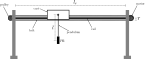
\includegraphics[width=\textwidth]{systemSetup}
  \caption{The setup provided by AAU. The motor controller in use is not directly visible in this picture as it is mounted behind the power supply.}
  \label{fig:systemSetup}
\end{figure}

As seen in \autoref{fig:systemSetup} the belt is attracted by pulleys one of which is driven by a brushed Maxon 370356 DC motor \cite{maxonMotor}. An other of these maxon motors is mounted on the pendulum but is disconnected and just used as a bearing in this project. Both motors are fitted with an HEDS 5540 optical quadrature encoder allowing for relative position and angle of the cart and pendulum respectively \cite{avagoTechnologies}.

The motor driving the belt is controlled using a Maxon ADS 50/10 motor controller configured in current control mode. The motor controller takes a $\pm$\SI{10}{V} input signal which then determines the armature current, $i_a$, see \cite{maxonMotorController}.

The primary control unit is a Teensy 3.6 microcontroller board. To program the board through the onboard USB connection a bootloader is used along with the Teensyduino add-on for the Arduino IDE \cite{sprkfunTeensy}.

The encoders are decoded on a shield using Avago HCTL-2021-PLC decoders and read through an 8 bit parallel data bus on the microcontroller board resulting in 2000 tics pr. revolution. This ensures a resolution for the pendulum angle, $\theta$, of $2\pi/2000=$ \SI{\pi e-3} rad/tic and $2\pi r /2000=\nolinebreak 2\pi\cdot 0.028 /2000\approx$ \SI{0.088e-3} m/tic for the cart position, $x$, see \cite{avagoDataSheet}.

The supply circuit on the microcontroller board is powered by 5V which is regulated to \SI{3.3}{V} resulting in a $0-$\SI{3.3}{V} range for the 12 bit analog output \cite{teensyDataSheet}. This output is used to provide the motor controller with an armature current reference, thus, the microcontroller analog output is amplified through the shield to meet the $\pm$\SI{10}{V} input requirement of the motor controller \cite{JHHorgensen}.

The following relation between analog 12 bit output values, $\text{bit}_\text{DAC}$, from the microcontroller and armature current in the motor was found by a previous project group \cite{JHHorgensen}, %linear regression
%
\begin{align}
  \text{bit}_\text{DAC} &= 105.78 \cdot i_{a} + 1970  \ \ \ , 
  \label{eq:Ia-bit}
\end{align}
%
and as a result of a force test, see \cite{NSVestergaard}, \autoref{eq:Ia-bit} was corrected to,
\begin{align}
  \text{bit}_\text{DAC} &= 111.9 \cdot i_{a} + 1970  \ \ \ ,
  \label{eq:Ia-bit-corrected}
\end{align}
which is the relation used in this project.
All the system parameters used in the design are listed in \autoref{table:systemParameters}. It is assumed that all frictions in the system can be modeled as a combination of Coulomb and viscous frictions. Wires hanging from the cart are unmodeled and their weight along with that of the belt are contained in the estimation of the cart mass. 

\begin{table}[H]
  \begin{tabular}{|l|l|l|l|}
    \hline %-----------------------------------------------------------------------------------------
    \textbf{Parameter}        & \textbf{Notation} & \textbf{Quantity} & \textbf{Unit}              \\
    \hline %-----------------------------------------------------------------------------------------
    Nominal current
    (max. continuous current) & $I_{\mathrm{N}}$  & \SI{4.58}         &  \si{A}                    \\
    \hline %-----------------------------------------------------------------------------------------
    Torque constant           & $\tau_m$          & \SI{93.4e-3}      &  \si{N\cdot m\cdot A^{-1}} \\
    \hline %-----------------------------------------------------------------------------------------
    Pendulum Rod Length       & $l$               & \num{0.3169}      &  \si{m}                    \\
    \hline %-----------------------------------------------------------------------------------------
    Rail Length               & $l_r$             & \num{0.89}        &  \si{m}                    \\
    \hline %-----------------------------------------------------------------------------------------
    Pulley Radius             & $r$               & \num{0.028}       &  \si{m}                    \\
    \hline %-----------------------------------------------------------------------------------------
    Pendulum Mass             & $m$               & \num{0.2235}      &  \si{kg}                   \\
    \hline %-----------------------------------------------------------------------------------------
    Cart Mass                 & $M$               & \num{6.28}        &  \si{kg}                   \\
    \hline %-----------------------------------------------------------------------------------------
    Cart Coulomb Friction     & $b_{c,c}$         & $f(x,\dot{x})$    &  \si{N}                    \\
    \hline %-----------------------------------------------------------------------------------------
    Cart Viscous Friction     & $b_{c,v}$         & \num{0}           &  \si{N\cdot m^{-1}\ s}      \\
    \hline %-----------------------------------------------------------------------------------------
    Pendulum Coulomb Friction & $b_{p,c}$         & \SI{4.1e-3}       &  \si{N\cdot m}             \\
    \hline %-----------------------------------------------------------------------------------------
    Pendulum Viscous Friction & $b_{p,v}$         & \SI{0.5e-3}       &  \si{N\cdot m\cdot s}      \\
    \hline %-----------------------------------------------------------------------------------------
  \end{tabular}
  \caption{The motor parameters, $I_{\mathrm{N}}$ and $\tau_m$, are given by maxon in \cite{maxonMotor}. The rod length is measured from the pendulum pivot point to the geometrical center of the pendulum mass. Pulley radius, rail length, pendulum mass and rod length, are measured parameters, while cart mass is estimated same as all frictions. The cart Coulomb friction turns out to be a function of the cart position in addition to velocity. Details on parameter estimation are found in the implementation section at the end of \textit{Part 1}.\label{table:systemParameters} }
\end{table}
%The estimations are performed by a previous project group \cite{JHHorgensen}.

\section{Model}\label{sec:model}
The model is based on the generalized coordinates presented in \autoref{fig:mechanicalDrawing}.
\begin{figure}[H]
  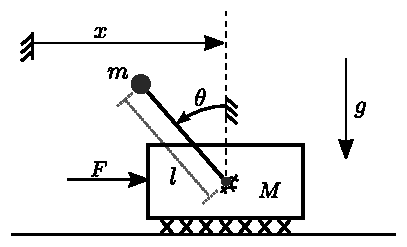
\includegraphics[width=.35\textwidth]{figures/mechanicalDrawing}
  \caption{Mechanical drawing of the system, where $\theta$ is the angle of the pendulum, $x$ is the position of the center of the cart along the rail, $F$ is the applied force and $g$ is the gravitational acceleration. It is indicated that friction is modeled between cart and rail as well as in the pendulum joint.}
  \label{fig:mechanicalDrawing}
\end{figure}
The pendulum mass center is positioned at zero hight at rest s.t. all energies in the system are positive. It is assumed that the pendulum rod is rigid and massless and that the pendulum weights are a point mass at the geometrical center of the weights.\\
The motor torque is given by direct relation to the armature current by the motor constant, $\tau_m = k_\tau i_a $, such that,
\begin{align}
  F &= \tfrac{1}{r} k_\tau i_a  \ \ \ .
\label{eq:motorForce}
\end{align}
%
To avoid excessive notation $u=F$ is considered to be the control input in the remaining of this thesis, while keeping in mind the relation in \autoref{eq:motorForce} along with the knowledge that $u$ must be converted to armature current in implementation.

%\begin{align}
%&& F &= \tfrac{1}{r} k_\tau i_a  &a
%\label{eq:motorForce}
%\end{align}
%
It is well known that the potential energy, $U$, and the kinetic energy, $T$, are given by, \cite{RWisniewski}
\begin{align}
  U &= mgl( 1 + \cos \theta )   \\
  T &= \frac{1}{2} ( M + m ) \dot{x}^2 - m \dot{x} l \cos \theta \dot{\theta} + \frac{1}{2} m l^2 \dot{\theta}^2 \ \ \ .
  \label{eq:generalizedPotentialAndKinetic}
\end{align}
The frictions, indicated in \autoref{fig:mechanicalDrawing}, are, as mentioned, comprised of Coulomb and viscous frictions with values stated in \autoref{table:systemParameters}. The viscous frictions are modeled as linear functions of velocities, \cite{CMClose, HOlsson}
\begin{align}
  b_{p,v} \dot{\theta} \ \ \ , & \ \ \ \ \ b_{c,v} \dot{x} \ \ \ , 
\label{eq:viscousFrictions}
\end{align}
for the rotational and linear case respectively.
The coulomb frictions are modeled as a constant with its sign depending on the signs of the velocities, such that, \cite{CMClose, HOlsson}
\begin{align}
  \mathrm{sgn}(\dot{\theta}) b_{p,c} \ \ \ , & \ \ \ \ \  \mathrm{sgn}(\dot{x}) b_{c,c} \ \ \ .
\label{eq:coloumbFrictions}
\end{align}
This, however, introduces discontinuities at zero velocities. Thus, tanh-functions are used to obtain a continues approximation of the sign-functions,
\begin{align}
  \tanh(\text{k}_\text{tanh}\dot{\theta}) b_{p,c} \ \ \ , & \ \ \ \ \ b_{c,v} \dot{x} - \tanh(\text{k}_\text{tanh}\dot{x}) b_{c,c} \ \ \ ,
\label{eq:coloumbFrictionsTanh}
\end{align}
where $\text{k}_\text{tanh}=250$ to increase the steepness of the tanh-functions thereby obtaining a closer approximation of the sign-functions.
Finally, by use of the Lagrange-d’Alembert Principle, \cite{RWisniewski}
\begin{align}
  \frac{d}{dt}  \frac{\partial \cal{L}}{\partial \dot{\vec{q}}} - \frac{\partial \cal{L}}{\partial \vec{q}}  &=  \vec{Q} \ \ \ ,
  \label{eq:energyMethodWithExternalForces}
\end{align}
\begin{align}
  \vec{q} &= 
  \begin{bmatrix}
    \theta    \\
    x
  \end{bmatrix} \ \ \ , \ \ \ 
  \vec{Q} =
  \begin{bmatrix}
    -b_{p,v} \dot{\theta} - \tanh(\text{k}_\text{tanh}\dot{\theta}) b_{p,c}    \\
    \tfrac{1}{r} k_\tau i_a - b_{c,v} \dot{x} - \tanh(\text{k}_\text{tanh}\dot{x}) b_{c,c}
  \end{bmatrix} \ \ \ ,
  \label{eq:qAndQ}
\end{align}
and $\cal{L} = T-U$, the dynamics of the system are found,
\begin{align}
  m l^2 \ddot{\theta} - m l \cos \theta \ddot{x} - m g l \sin \theta  &= -b_{p,v} \dot{\theta} - \tanh(\text{k}_\text{tanh}\dot{\theta}) b_{p,c} \label{eq:energyDerivedDynamicEquation2} \\
  ( M + m )\ddot{x} + m l \sin \theta \dot{\theta}^2 - m l \cos \theta \ddot{\theta}  &=  u - b_{c,v} \dot{x} - \tanh(\text{k}_\text{tanh}\dot{x}) b_{c,c} \ \ \ .
  \label{eq:energyDerivedDynamicEquation1}
\end{align}
By setting up the dynamic equations, \autoref{eq:energyDerivedDynamicEquation1} and \ref{eq:energyDerivedDynamicEquation2}, in the following manner,
%
\begin{align}
\begin{split}
  &
  \begin{bmatrix}
    m l^2              & -m l \cos \theta  \\
    -m l \cos \theta   & M + m
  \end{bmatrix}
  \begin{bmatrix}
    \ddot{\theta}  \\
    \ddot{x}
  \end{bmatrix}
  +
  \begin{bmatrix}
    0  \\
    m l \sin \theta \dot{\theta}^2
  \end{bmatrix}
  +   \\
  &+
  \begin{bmatrix}
    b_{p,v} \dot{\theta} + \tanh(\text{k}_\text{tanh}\dot{\theta}) b_{p,c}    \\
    b_{c,v} \dot{x} + \tanh(\text{k}_\text{tanh}\dot{x}) b_{c,c}
  \end{bmatrix}
  +
  \begin{bmatrix}
    -m g l \sin \theta  \\
    0
  \end{bmatrix}
  =
  \begin{bmatrix}
    0  \\
    u
  \end{bmatrix} \ \ \ , 
\end{split}
\label{eq:thetaXdynamics}
\end{align}
%
the general form of an m-link robot is obtained, \cite{MWSpong, LSciavicco}
\begin{align}
  \vec{M}(\vec{q})\vec{\ddot{q}} + \vec{C}(\vec{q},\vec{\dot{q}}) + \vec{B}(\vec{\dot{q}}) + \vec{G}(\vec{q}) &= \vec{F} \ \ \ , \hspace{3.3cm}
\end{align}
\begin{where}
  \va{ \vec{M}(\vec{q})  }{is the inertia matrix}                    {}
  \va{ \vec{C}(\vec{q},\vec{\dot{q}})  }{is the Coriolis and centrifugal effects}  {}
  \va{ \vec{B}(\vec{\dot{q}})          }{is the friction}                          {}
  \va{  \vec{G}(\vec{q})               }{is the force due to gravity}              {}
  \va{  \vec{F}                        }{is the input force vector \ \ \ .}        {}
\end{where}

Choosing $ [\ x_1\ \ x_2\ \ x_3\ \ x_4\ ]^\mathrm{T} = [\ \theta\ \ x\ \ \dot{\theta}\ \ \dot{x}\ ]^\mathrm{T} $ as states results in the following nonlinear state space representation,
%
\begin{align}
  \begin{bmatrix}
    \dot{x_1} \\
    \dot{x_2} \\
    \dot{x_3} \\
    \dot{x_4}
  \end{bmatrix}
&=
  \left[
    \begin{array}{c}
      x_3 \\
      x_4 \\
      \multirow{2}{*}{$ \vec{M}^{-1}(x_1) ( \vec{F} - \vec{C}(x_1,x_3) - \vec{B}(x_3,x_4) - \vec{G}(x_1) ) $}\\
      \phantom{eq}
    \end{array}
  \right]
  \label{eq:nonlinearStateSpace} \ \ \ ,
\end{align}
%
which is convenient when simulating the system. This representation is also used in the controller designs.


